\documentclass[a4paper]{article}
\usepackage[utf8]{inputenc}
\usepackage{amsmath}
\usepackage{graphicx}
\usepackage{indentfirst}
\usepackage{subfig}
\usepackage{float} % para usar [H]
%opening

\begin{document}

\noindent UNIVERSIDAD SIMÓN BOLÍVAR\\
Departamento de Cómputo Científico\\
CO-6612, Introducción a las redes neuronales\\
Tarea 3: Perceptrón multicapas\\
María Victoria Jorge\\
11-10495

\section{Regresión lineal}
Para este ejercicio se utilizó el algoritmo de descenso de gradiente. La capa oculta fue implementada con la función logística y la de salida con una función de activación lineal. Además, se utilizó como condición de parada 700 épocas, actualización de los pesos secuencial y una tasa de aprendizaje de 0.01. El entrenamiento se realizó con 60 datos y para probar la aproximación del modelo se usaron 10000 datos nuevos. Como métrica de \textit{performance} se tomará en cuenta el error cuadrático medio (ECM) para decidir cuál arquitectura se ajusta mejor a los datos.\\

En la figura \ref{fig:n1-2-3_train} se encuentran las gráficas del ECM para las arquitecturas con 1, 2 y 3 neuronas en la capa oculta. En esta gráfica puede observarse como en los tres casos el ECM va disminuyendo con el paso de las épocas, llegando en su punto mínimo a 29.3351 para n = 1, 22.4029 para n = 2 y 11.3470 para n = 3. Lo que lleva a pensar que entre estas tres arquitecturas con la que se obtuvo un mejor modelo fue con 3 neuronas en la capa oculta.

	\begin{figure}[H]
	  \centering
	  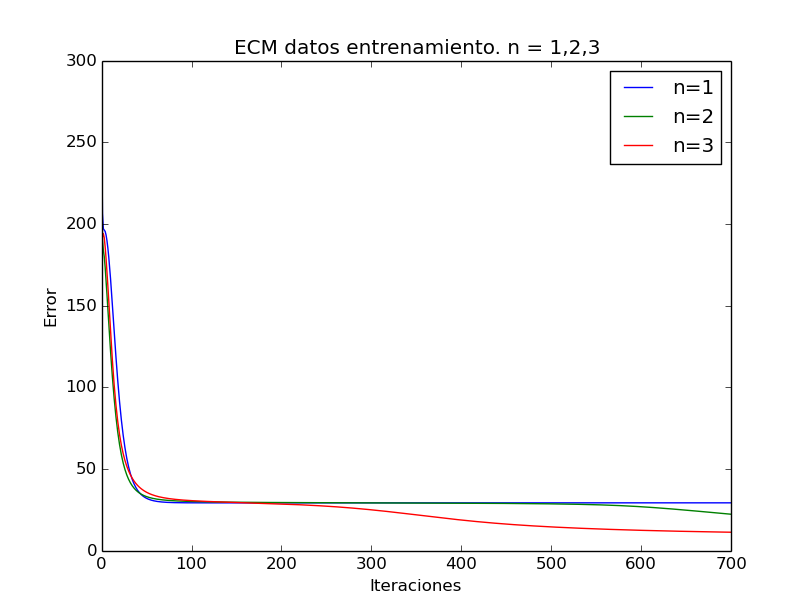
\includegraphics[scale=0.4]{graficas/n1-2-3_train.png}
	  \caption{ECM para n = 1,2,3}
	  \label{fig:n1-2-3_train}
	\end{figure}

Esto último también puede comprobarse con los resultados de probar el modelo con datos nuevos. La salida obtenida para los puntos no utilizados en la fase de entrenamiento se encuentra en la figura \ref{f:aprox1-2-3} para las tres arquitecturas mencionadas antes. Con ellas se puede apreciar que el modelo de \ref{f:n3_prueba} parece ajustarse mejor a la distribución de los datos, por lo que entre estos tres modelos, n = 3 es el mejor tomando como métrica el error.
	
	\begin{figure}[H]
	\centering
	\subfloat[$n=1$]{
	\label{f:n1_prueba}
	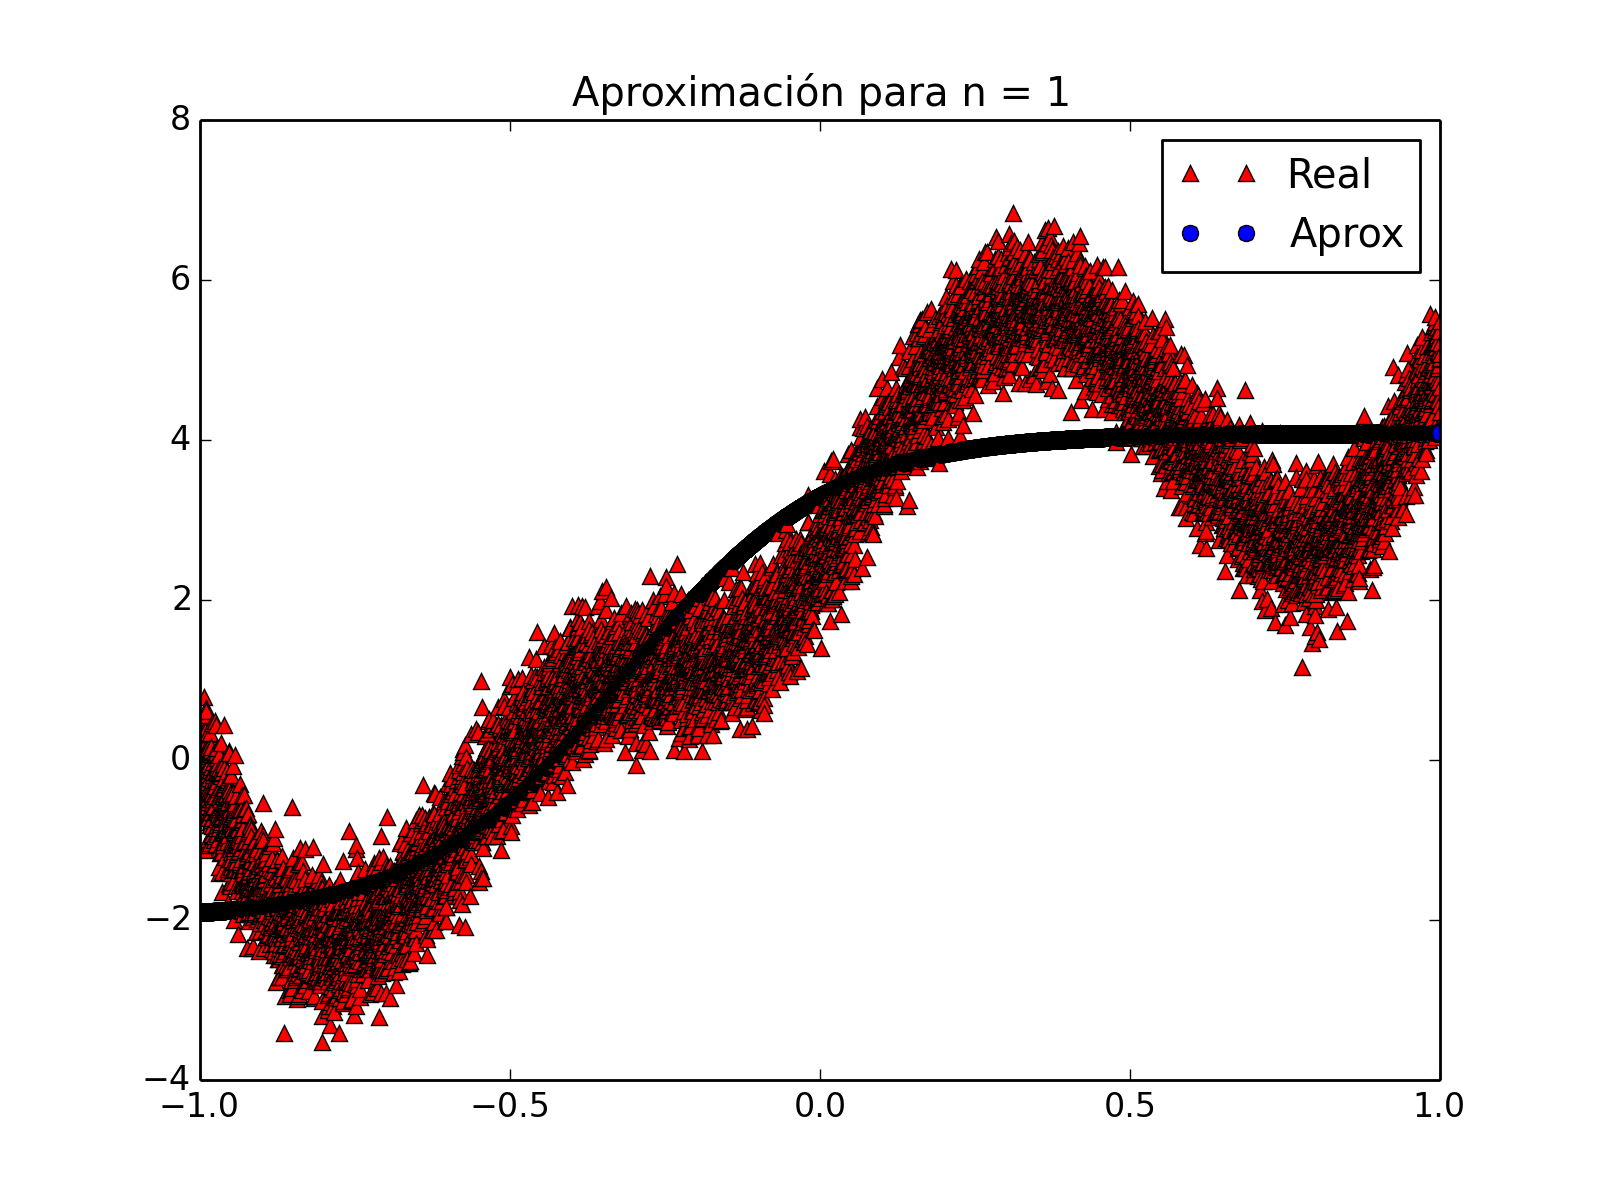
\includegraphics[width=0.5\textwidth]{graficas/n_1_prueba.png}}
	\subfloat[$n=2$]{
	\label{f:n2_prueba}
	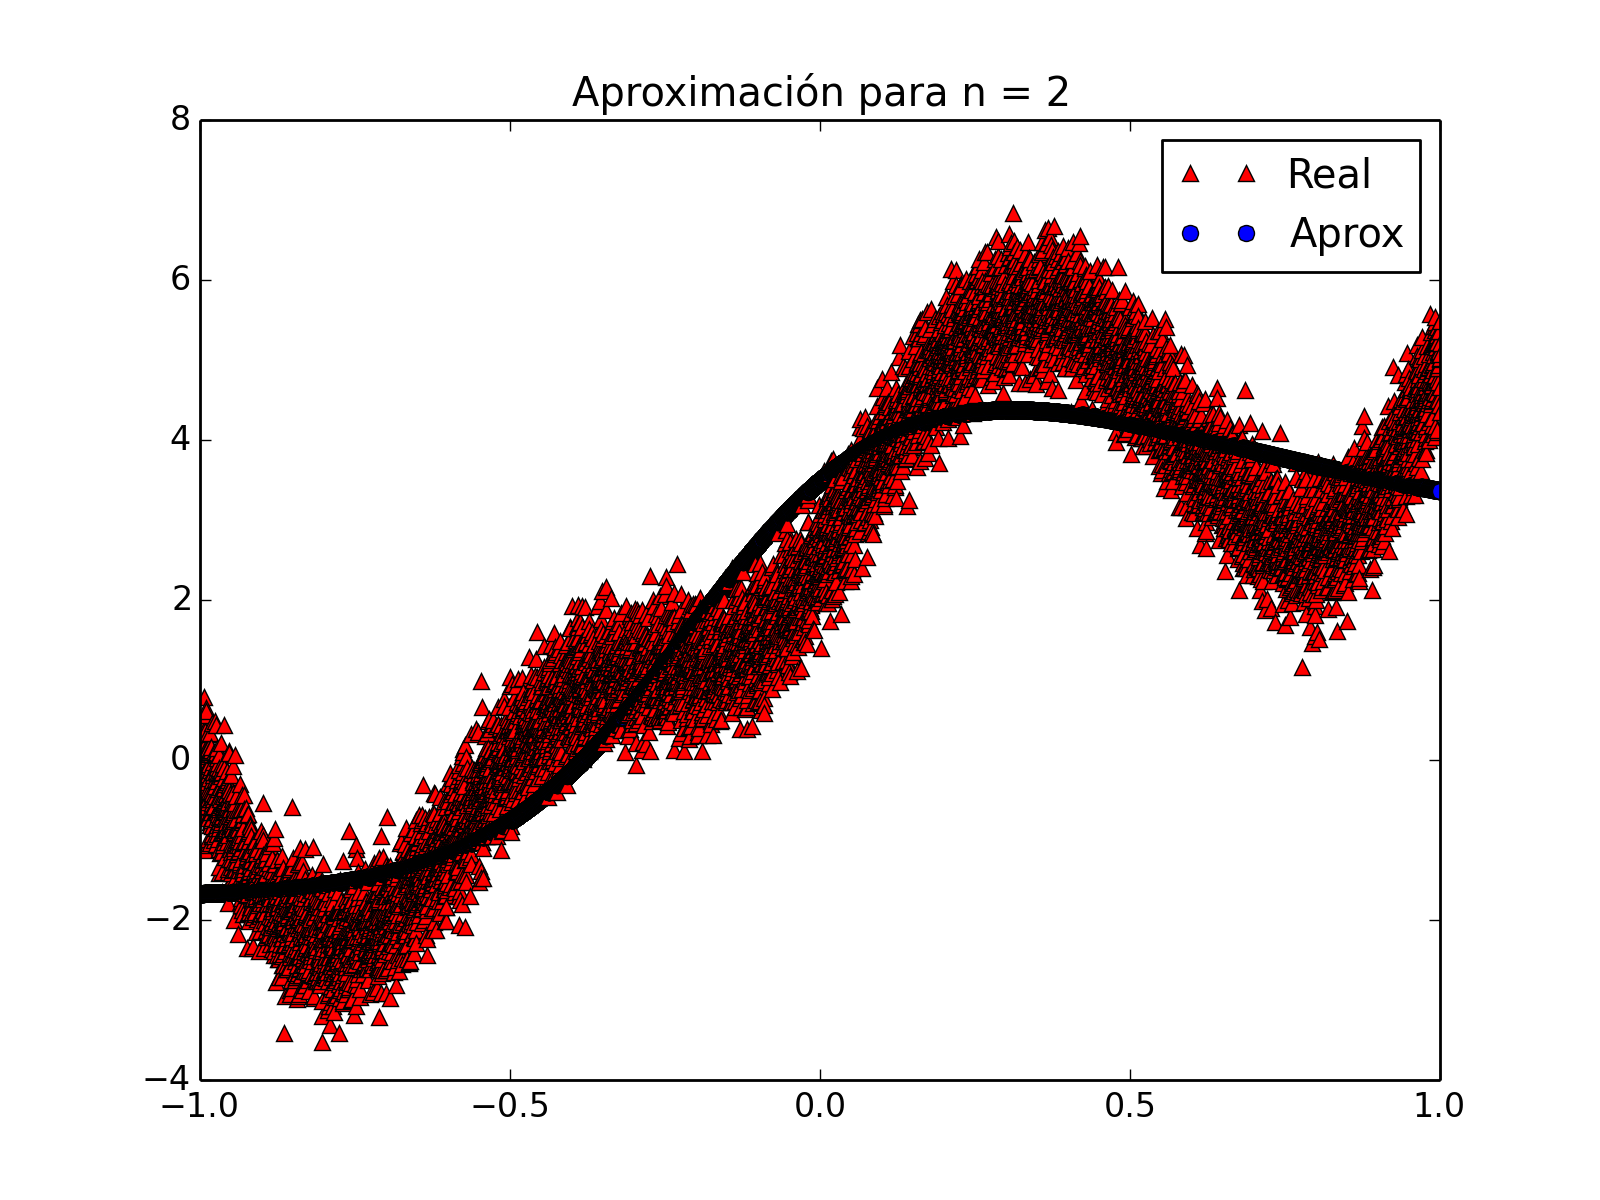
\includegraphics[width=0.5\textwidth]{graficas/n_2_prueba.png}}\\
	\subfloat[$n=3$]{
	\label{f:n3_prueba}
	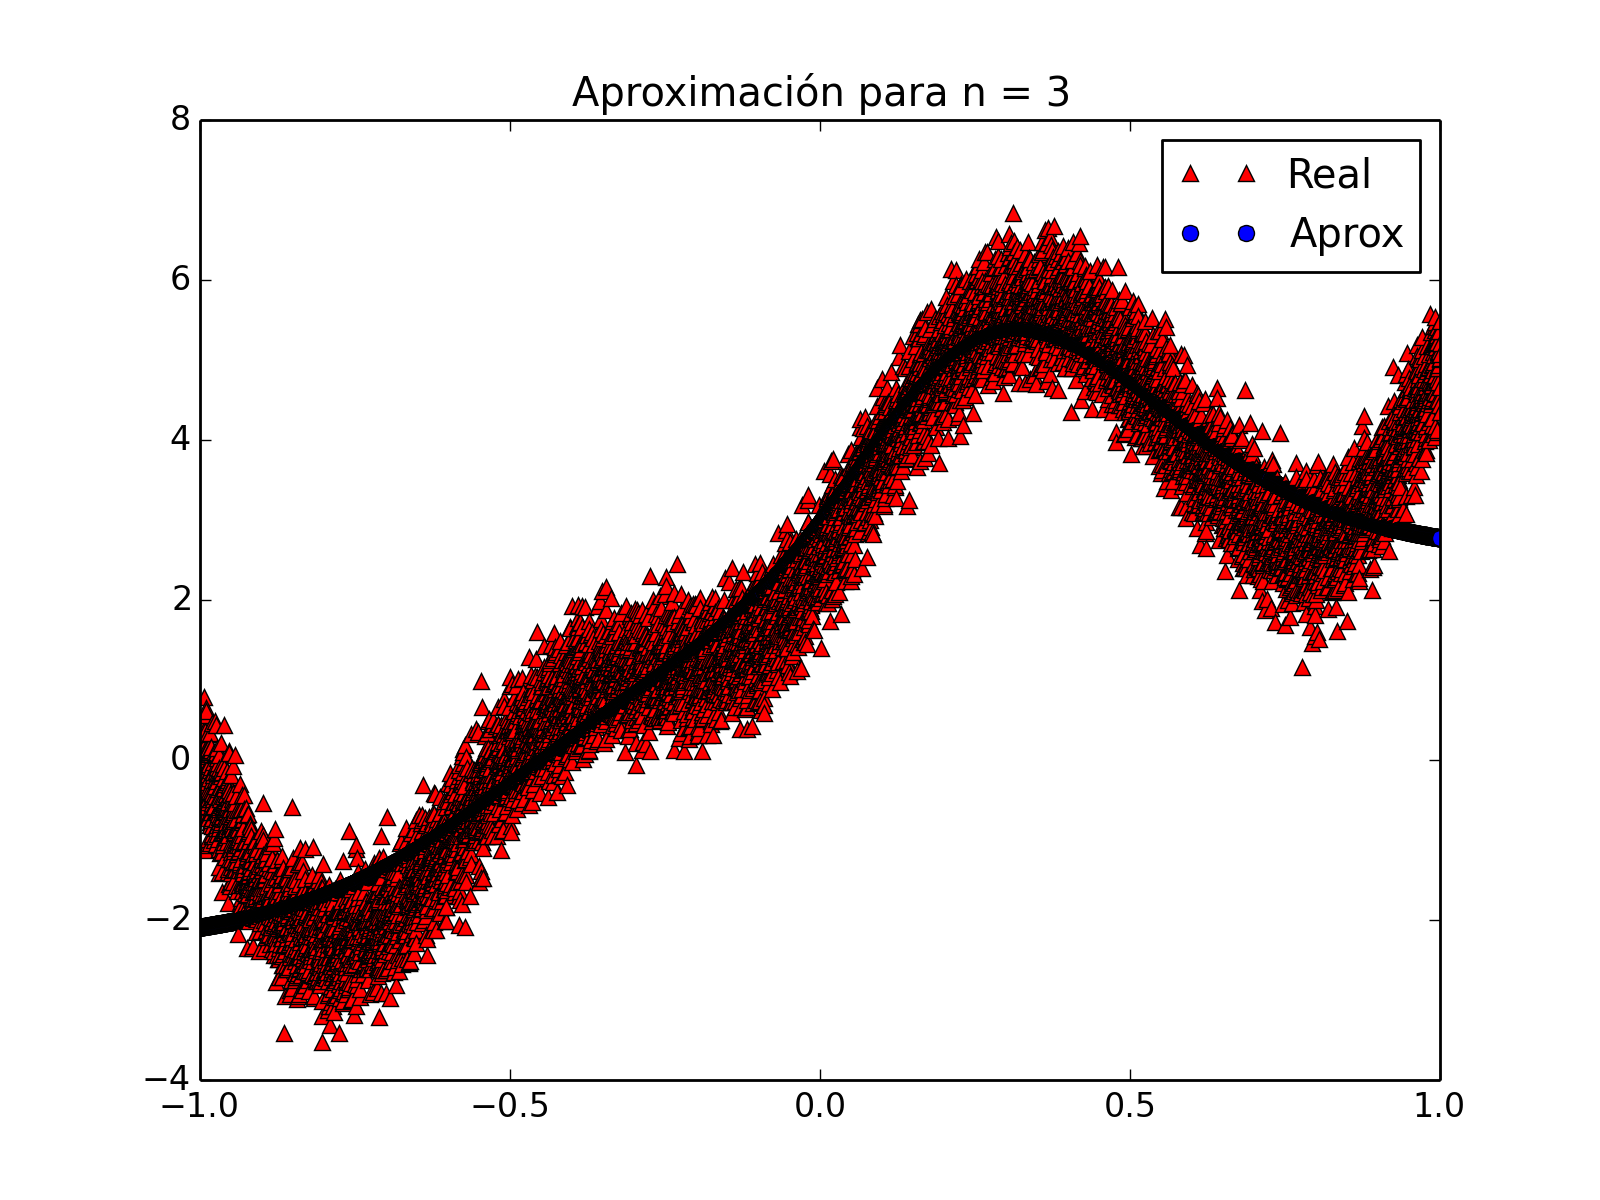
\includegraphics[width=0.5\textwidth]{graficas/n_3_prueba.png}}
	\caption{Modelos obtenidos para n = 1,2,3}
	\label{f:aprox1-2-3}
	\end{figure}

Aumentando la cantidad de neuronas ocultas a 4, 6 y 8 se obtuvieron los ECM presentes en la figura \ref{fig:n4-6-8_train}. El error mínimo obtenido para cada una de estas arquitecturas fue 11.5970, 11.8372 y 13.9363, respectivamente.
	
	\begin{figure}[H]
	\centering
	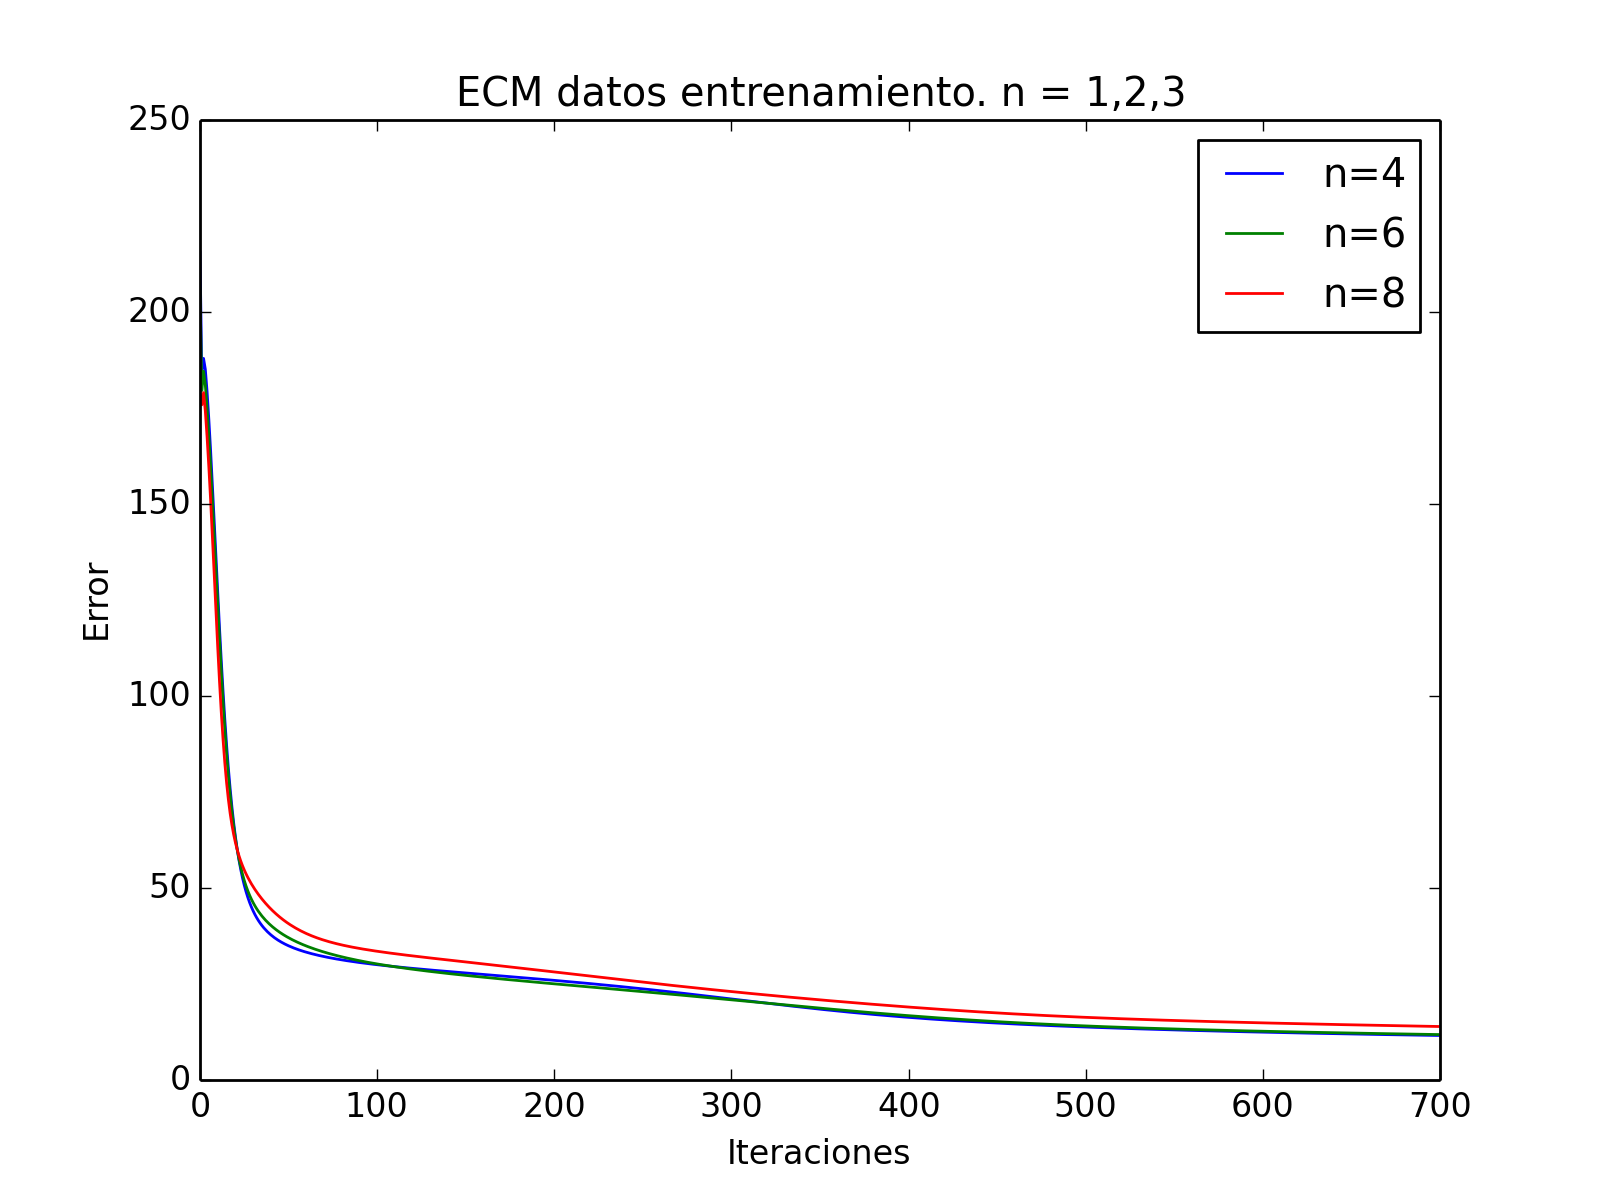
\includegraphics[scale=0.4]{graficas/n4-6-8_train.png}
	\caption{ECM para n = 4,6,8}
	\label{fig:n4-6-8_train}
	\end{figure}

Además, en la figura \ref{f:aprox4-6-8} se puede ver el comportamiento del modelo para estas arquitecturas con datos nuevos no usados para el entrenamiento. Tomando estas gráficas y los valores de ECM obtenidos, podemos ver que la arquitectura con 4 neuronas ocultas parece ser la que mejor generaliza el modelo, de las tres presentes.

	\begin{figure}[H]
	\centering
	\subfloat[$n=4$]{
	\label{f:n4_prueba}
	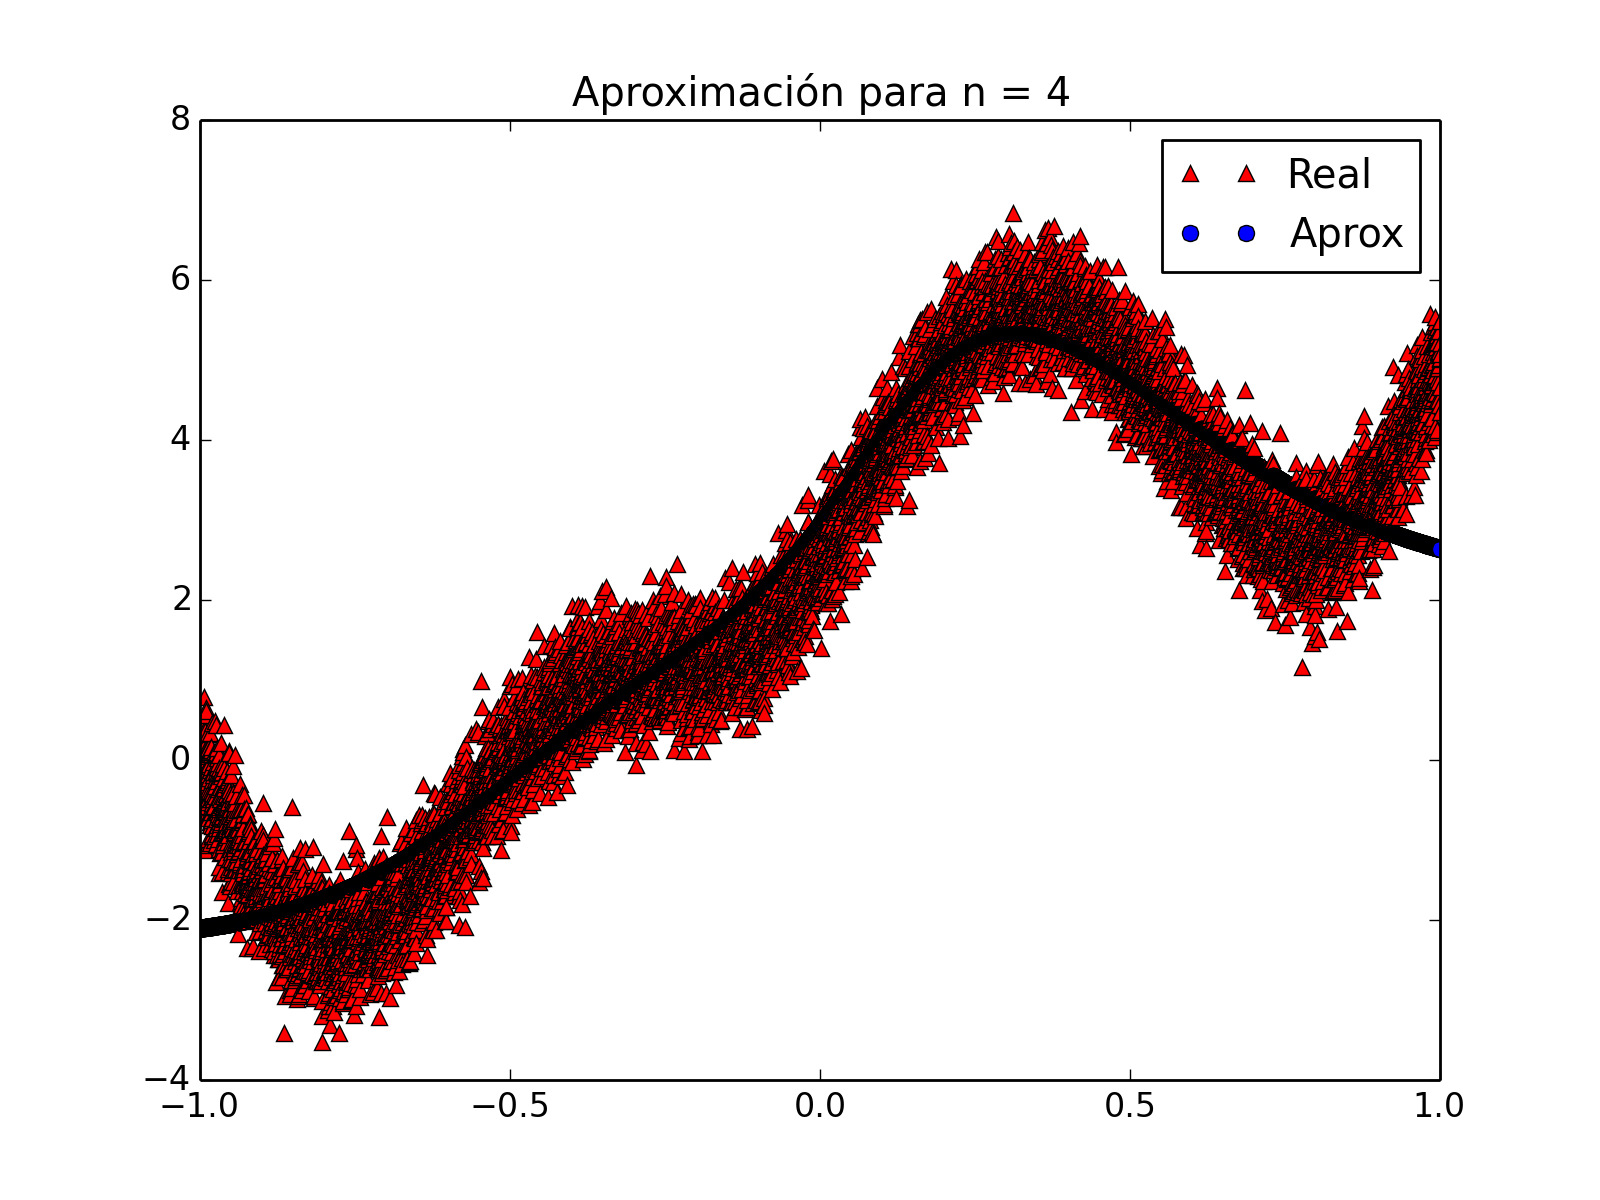
\includegraphics[width=0.5\textwidth]{graficas/n_4_prueba.png}}
	\subfloat[$n=6$]{
	\label{f:n6_prueba}
	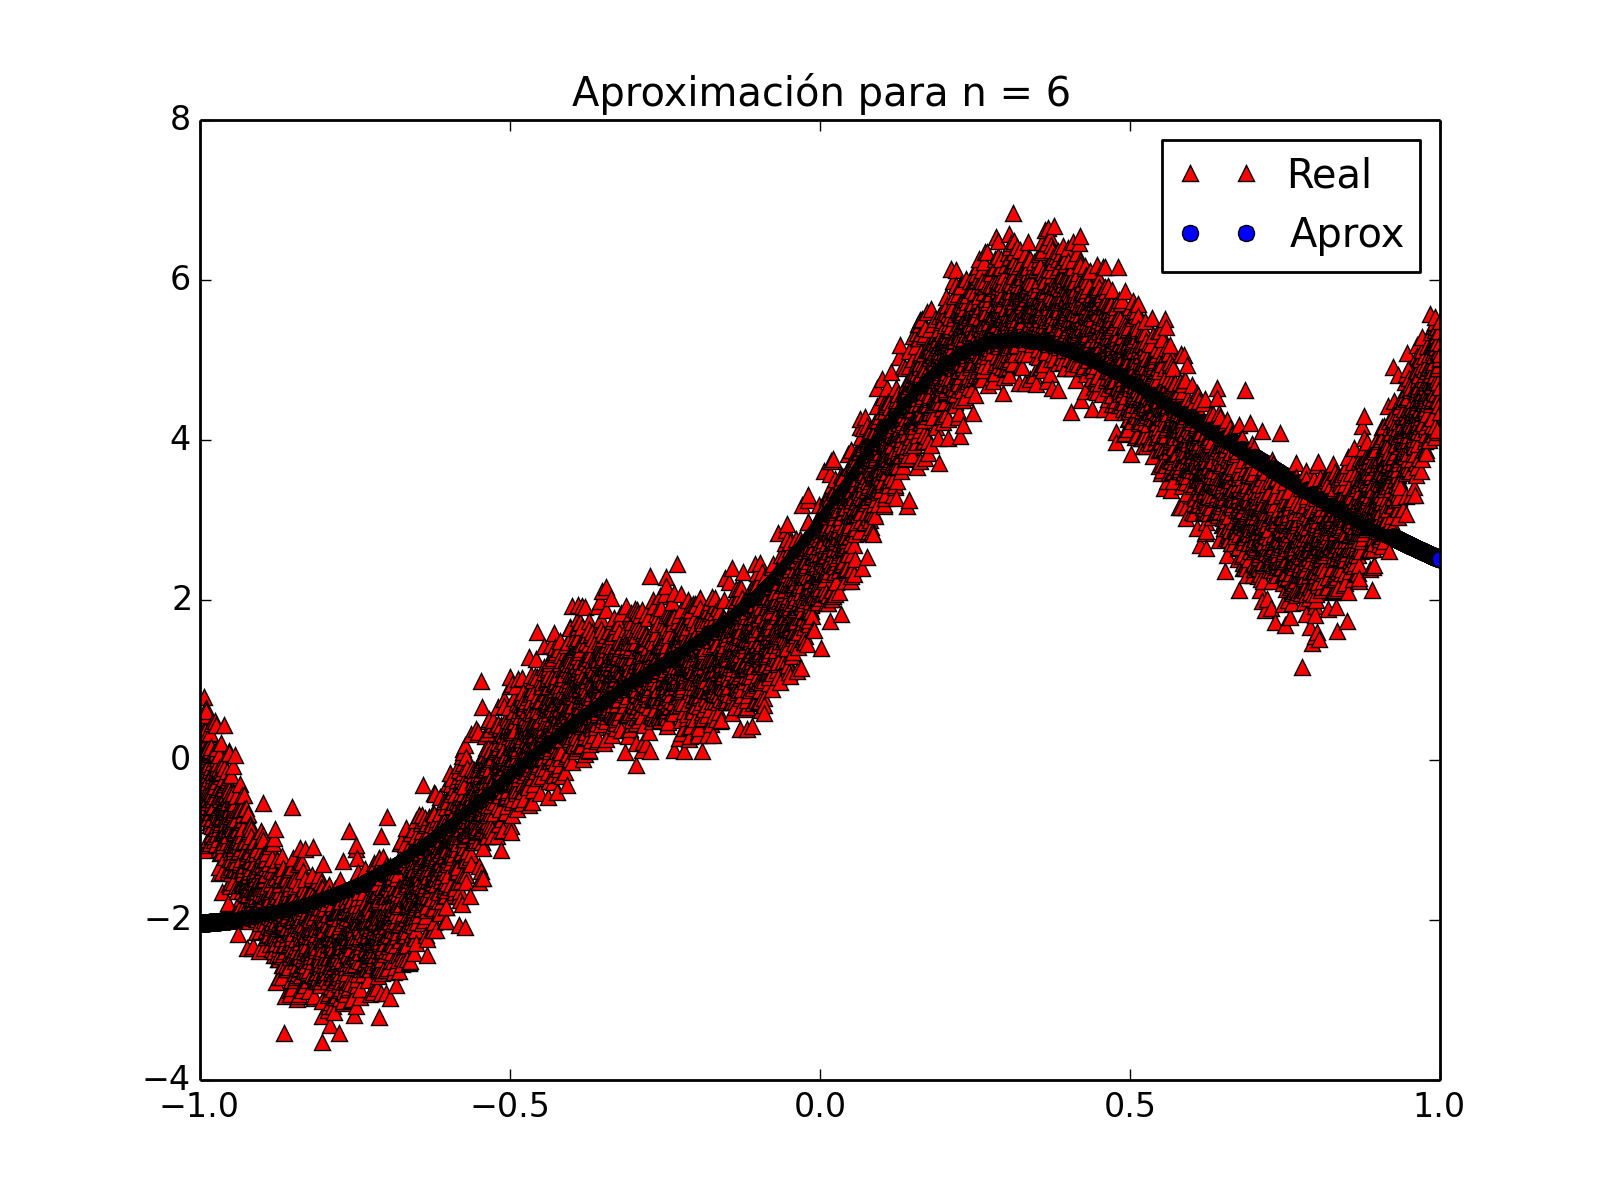
\includegraphics[width=0.5\textwidth]{graficas/n_6_prueba.png}}\\
	\subfloat[$n=8$]{
	\label{f:n8_prueba}
	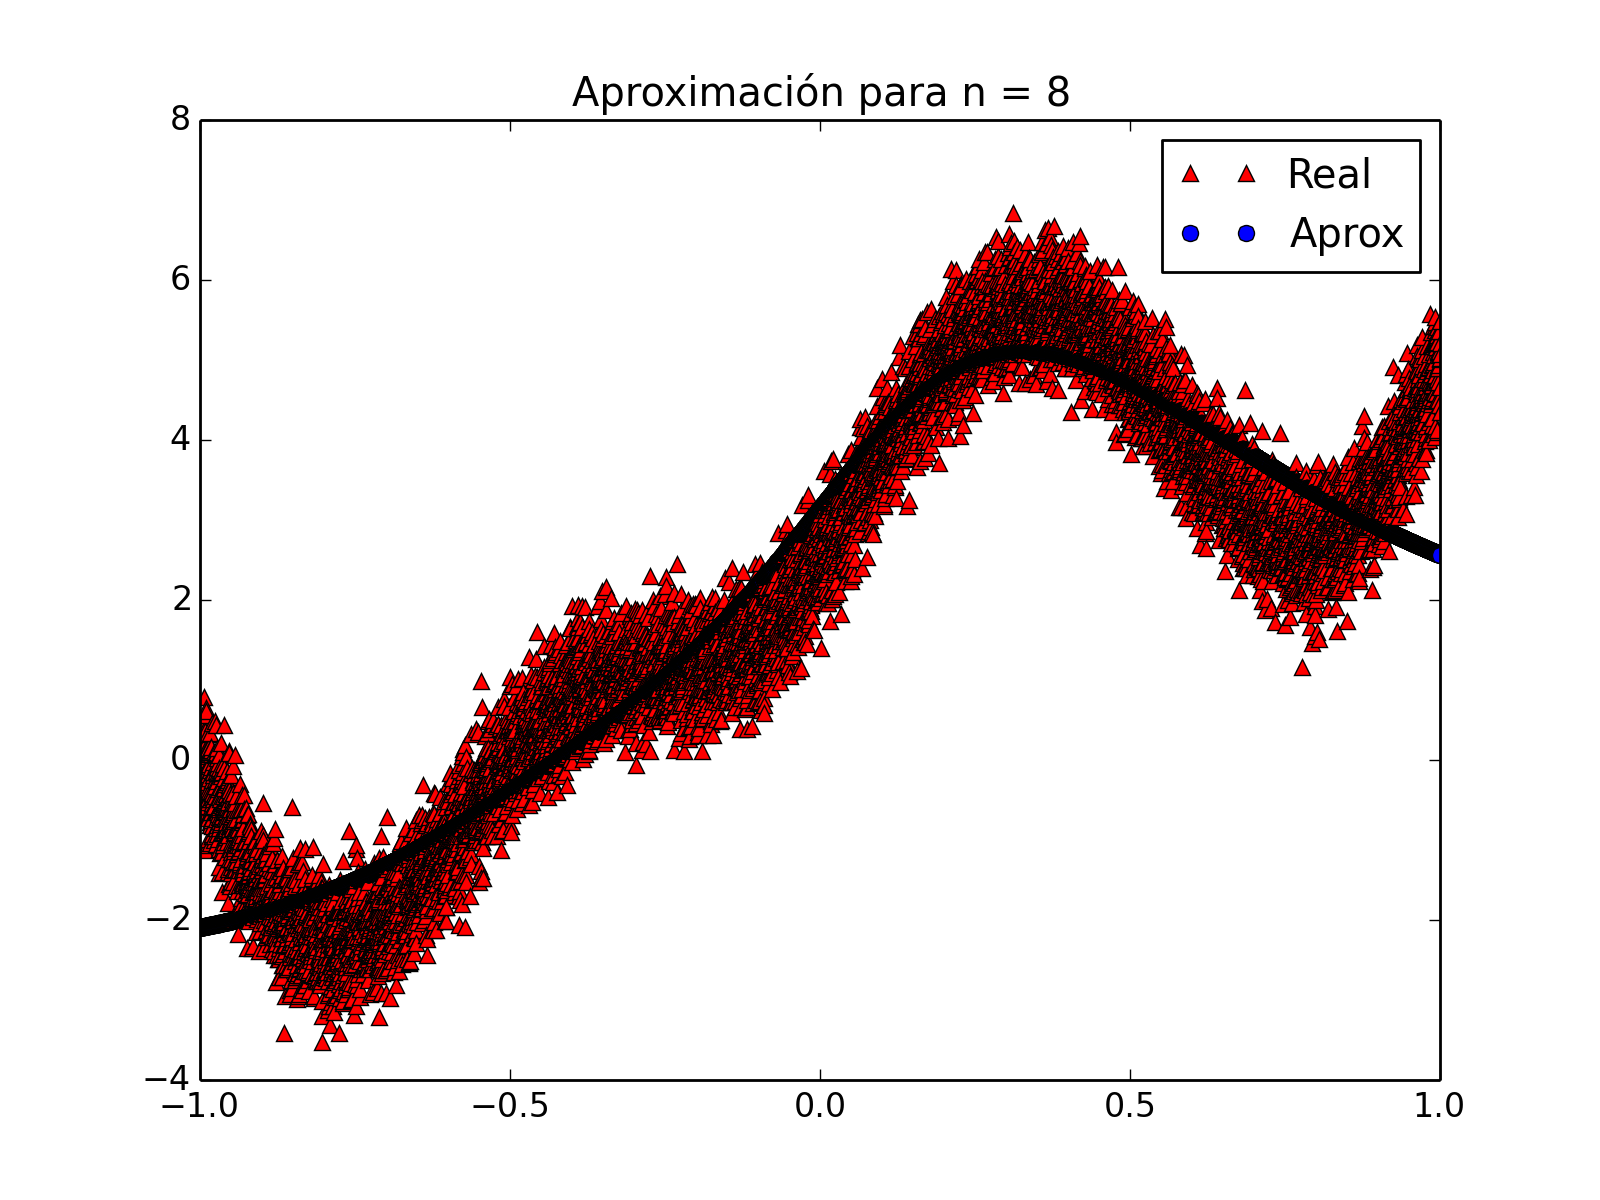
\includegraphics[width=0.5\textwidth]{graficas/n_8_prueba.png}}
	\caption{Modelos obtenidos para n = 4,6,8}
	\label{f:aprox4-6-8}
	\end{figure}

Finalmente, se realizaron experimentos con arquitecturas de 12, 20 y 40 neuronas ocultas. Los ECM obtenidos en cada caso se encuentran en la figura \ref{fig:n12-20-40_train}. El mínimo ECM obtenido al final de las 700 épocas para cada una de estas arquitecturas fue: 11.9803, 12.8926 y 13.5061, respectivamente.
	
	\begin{figure}[H]
	  \centering
	  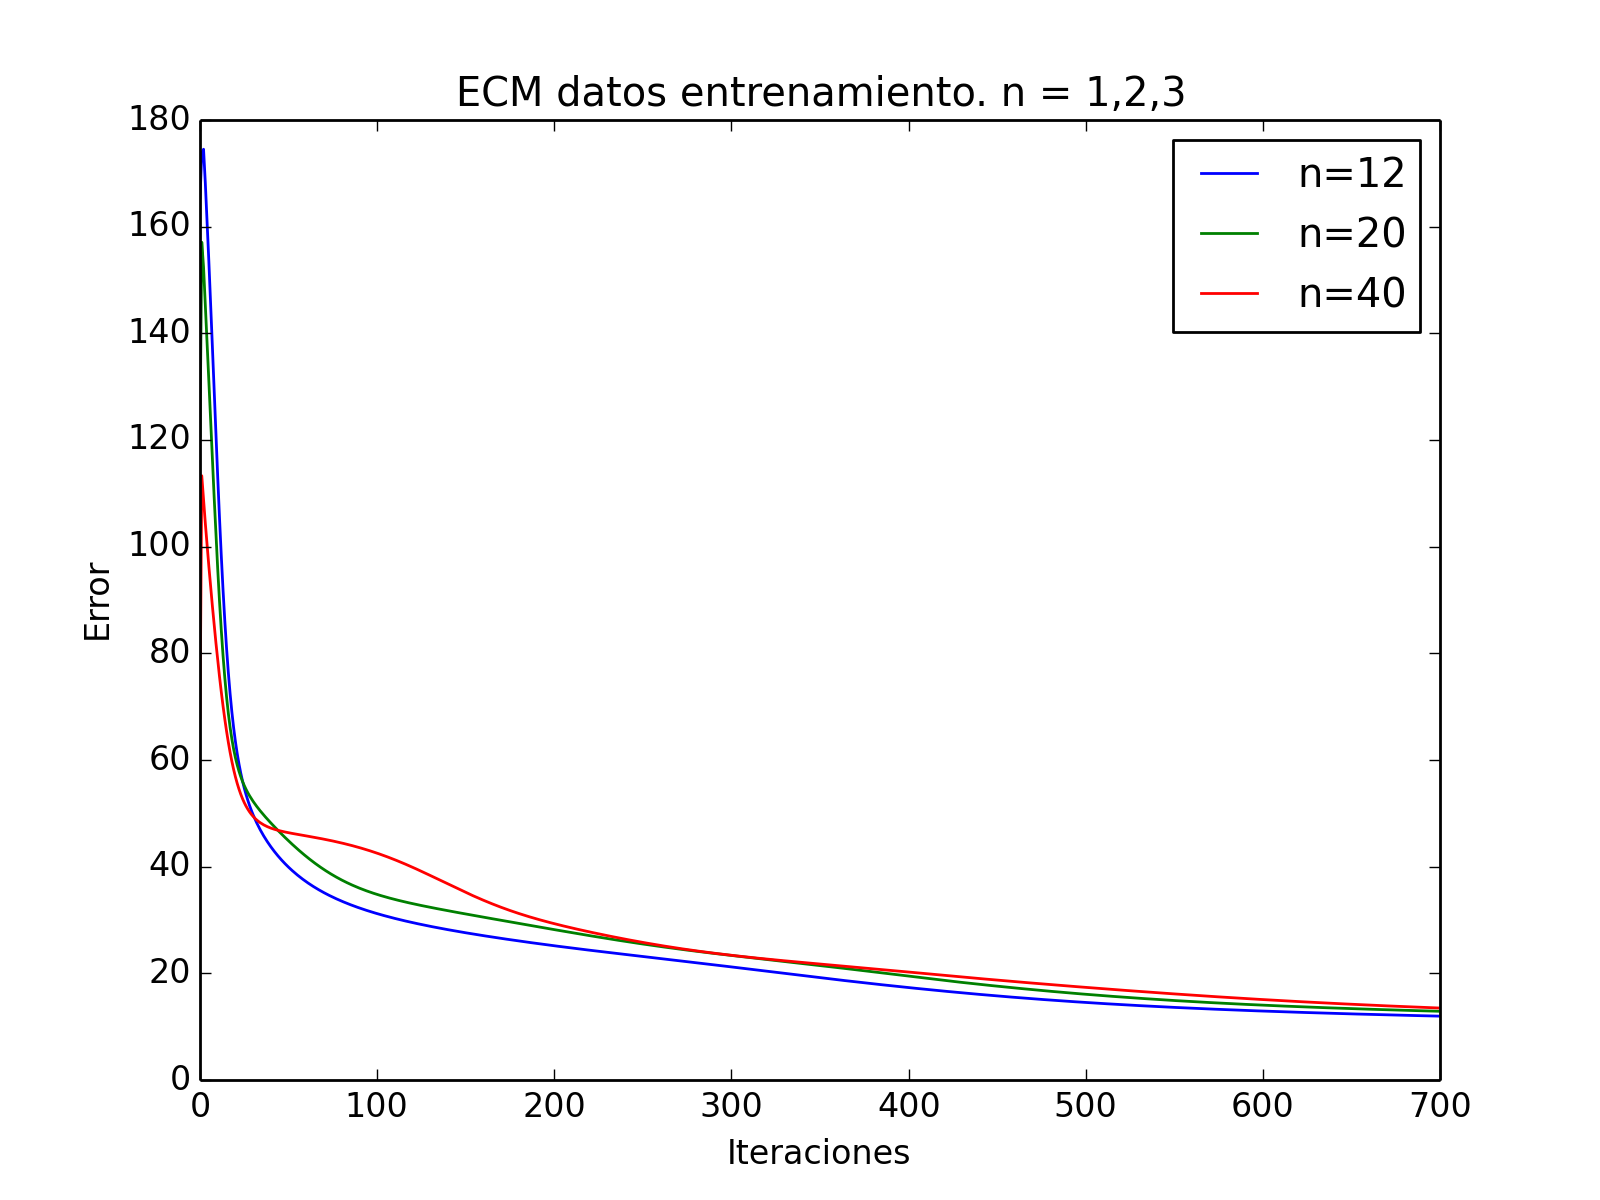
\includegraphics[scale=0.4]{graficas/n12-20-40_train.png}
	  \caption{ECM para n = 12,20,40}
	  \label{fig:n12-20-40_train}
	\end{figure}

Además, en la figura \ref{f:aprox12-20-40} se encuentran las aproximaciones con cada arquitectura usando datos nuevos. Con esta información y los ECM obtenidos para cada modelo, podemos ver que la mejor de estas tres arquitecturas es n = 12.

	\begin{figure}[H]
	\centering
	\subfloat[$n=12$]{
	\label{f:n12_prueba}
	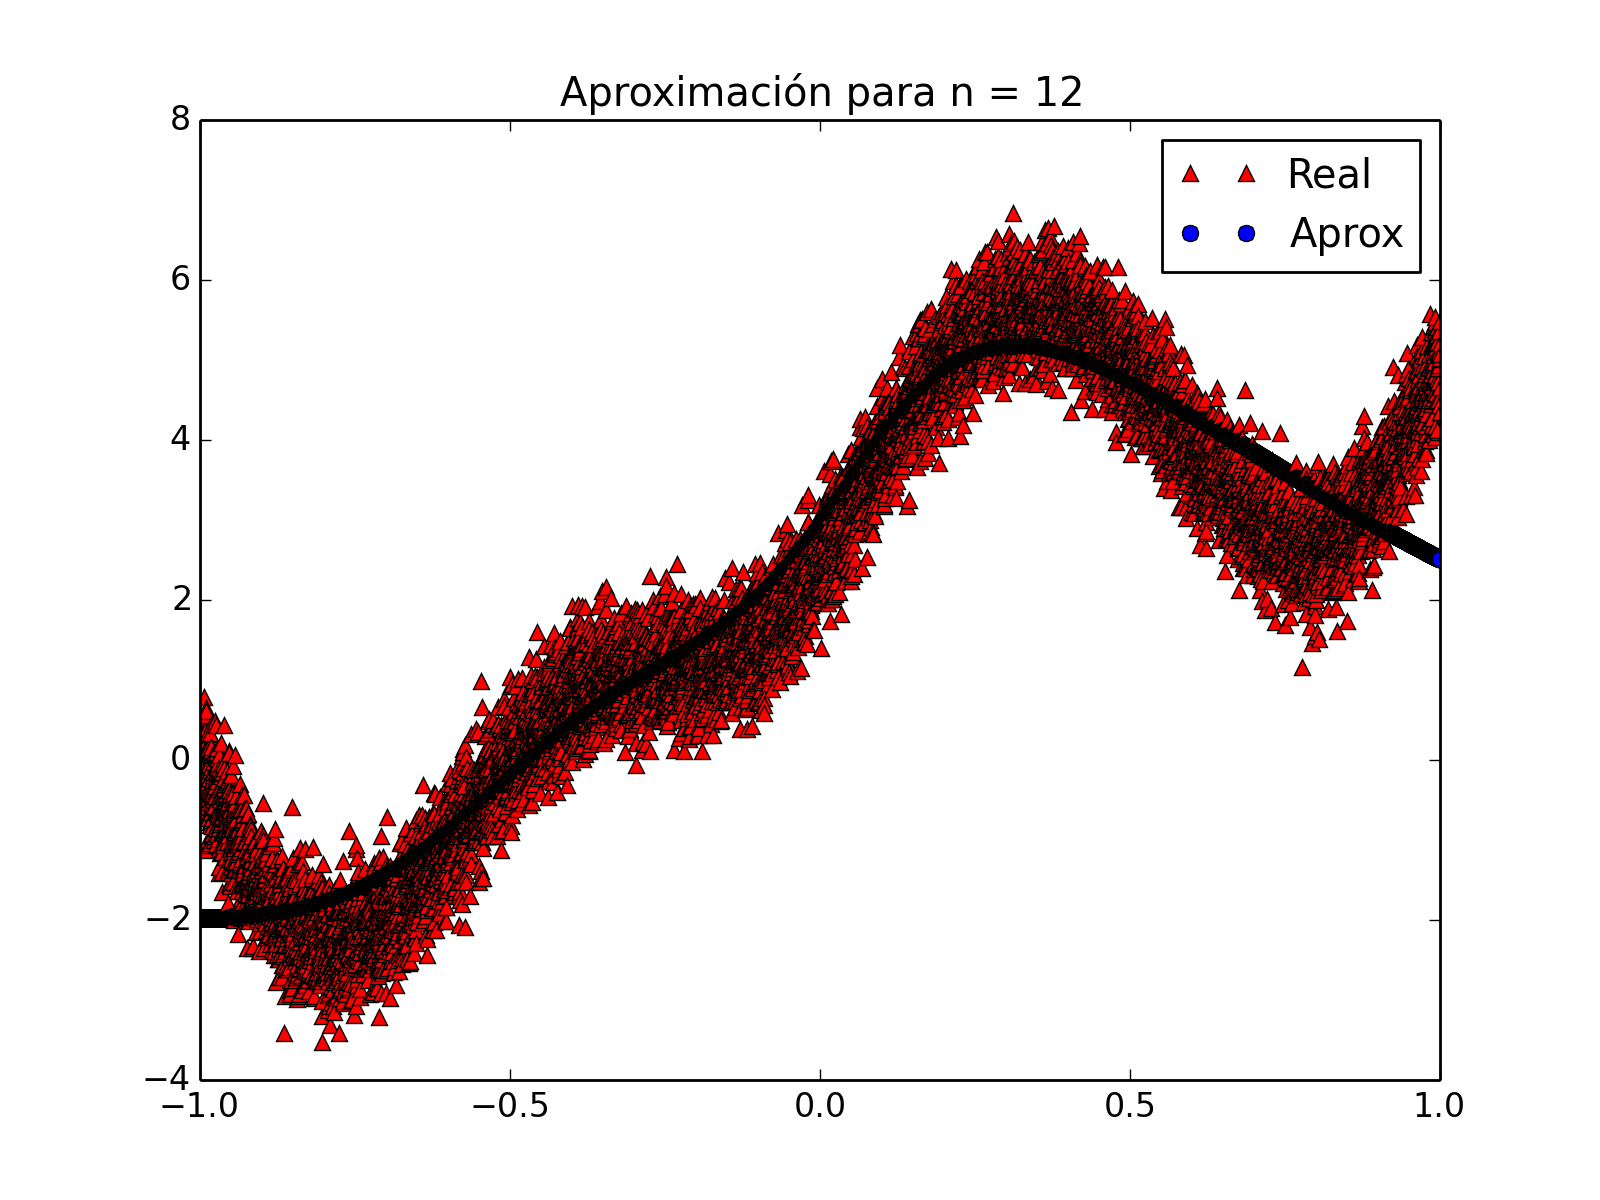
\includegraphics[width=0.5\textwidth]{graficas/n_12_prueba.png}}
	\subfloat[$n=20$]{
	\label{f:n20_prueba}
	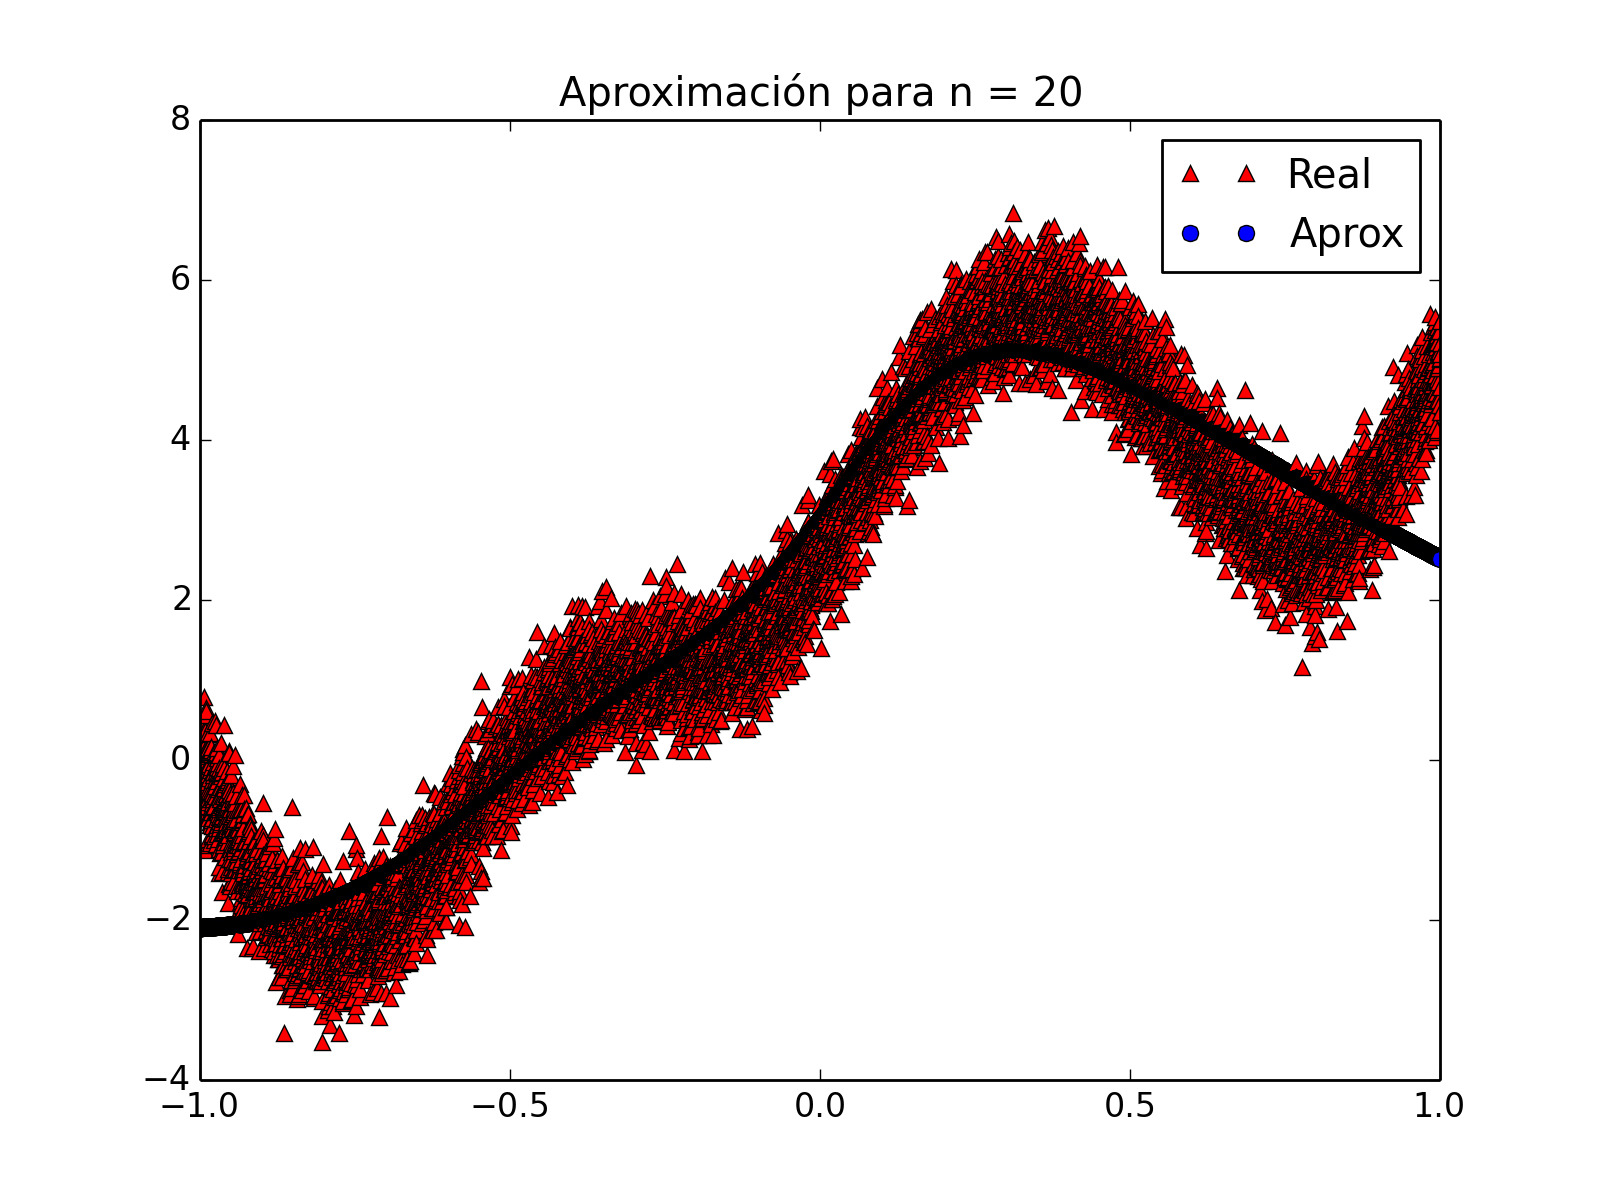
\includegraphics[width=0.5\textwidth]{graficas/n_20_prueba.png}}\\
	\subfloat[$n=40$]{
	\label{f:n40_prueba}
	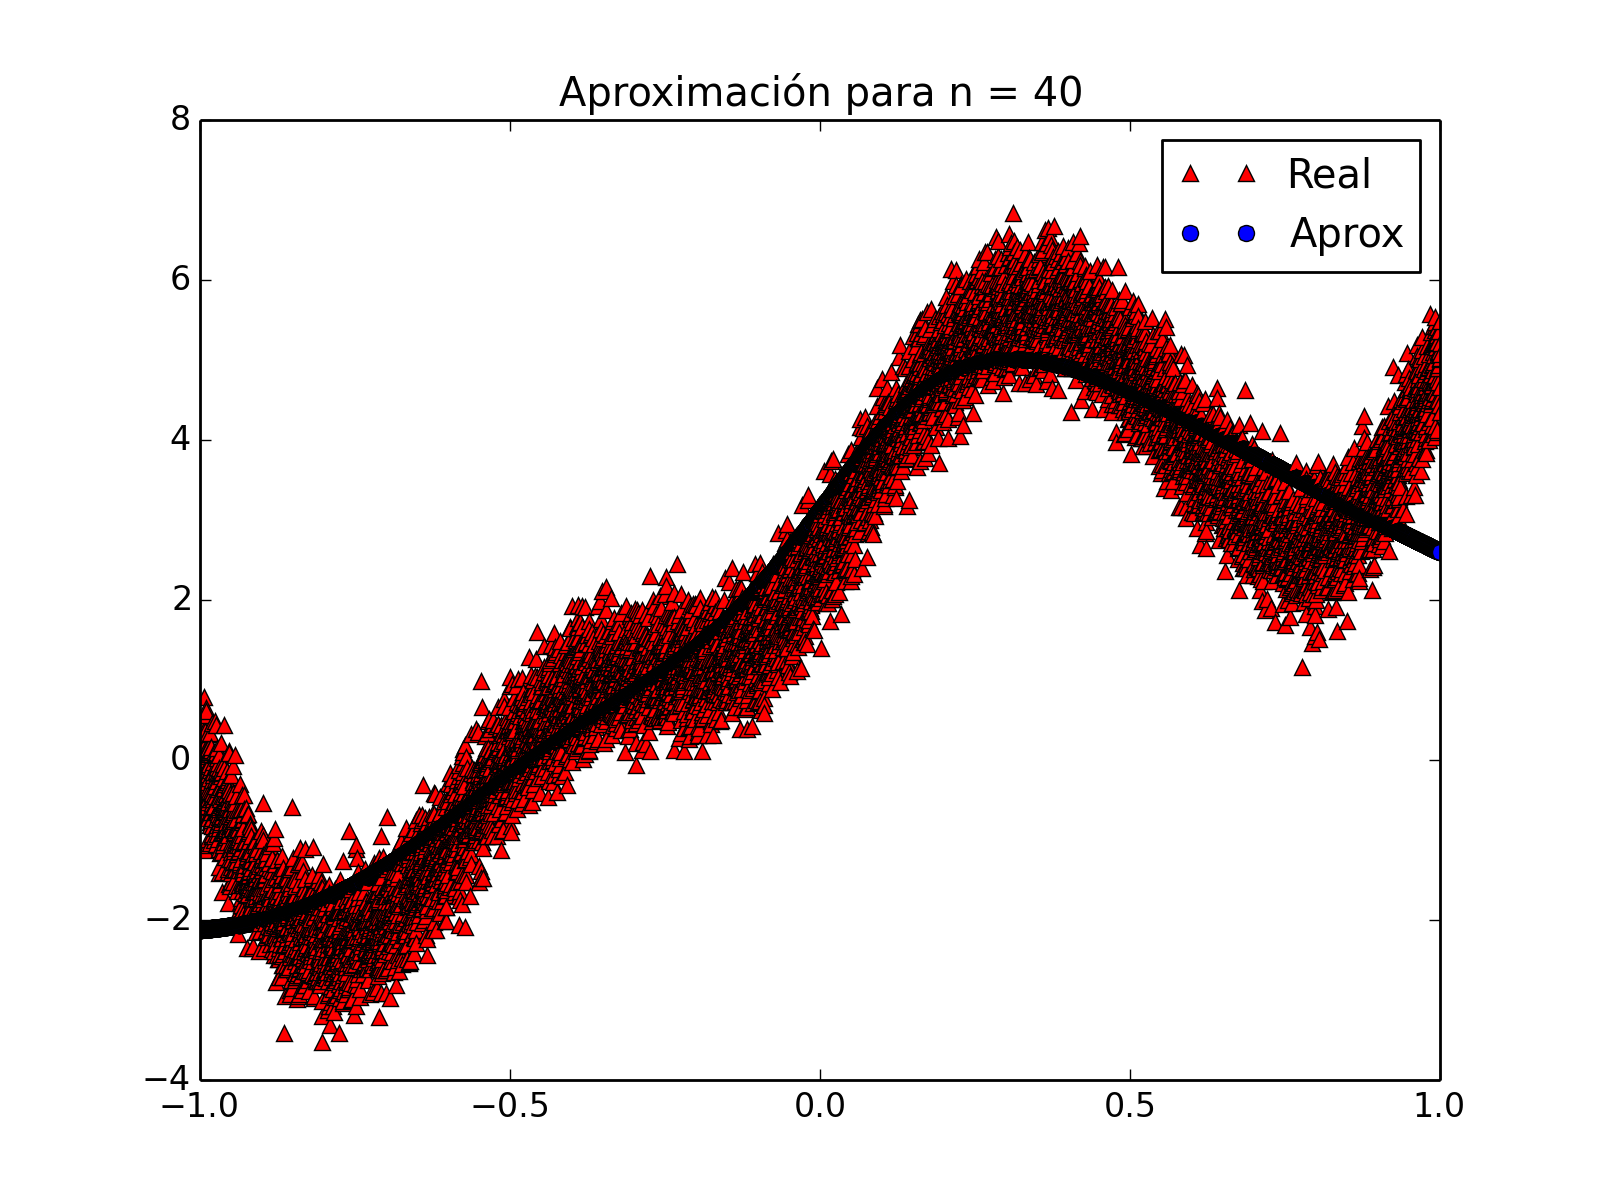
\includegraphics[width=0.5\textwidth]{graficas/n_40_prueba.png}}
	\caption{Modelos obtenidos para n = 12,20,40}
	\label{f:aprox12-20-40}
	\end{figure}
	
En conclusión, luego de realizar los experimentos en grupos de tres arquitecturas, se tiene que para cada grupo las mejores arquitecturas son n = 3, 4 y 12. Luego, tomando los ECM de las tres (11.3470, 11.5970 y 11.9803), tenemos que la arquitectura que parece aproximarse mejor al modelo de regresión lineal es la de 3 neuronas logísticas ocultas y una neurona lineal de salida.

\section{Dependencia del peso en conejos australianos}
Para lograr aproximar la dependencia entre el peso de los conejos australianos y su edad se realizarán experimentos sobre un MLP con los que se determinará la mejor tasa de aprendizaje, arquitectura de la red y número de épocas para la fase de entrenamiento. El algoritmo de aprendizaje que se utilizará es el de retropropagación, mismo que se usó en la pregunta anterior. Antes de usar las diferentes arquitecturas de MLP se normalizaron los datos para evitar generar saturación en las neuronas, dividiendo cada columna entre el máximo de la misma. Si no se realiza este preprocesamiento de los datos se produciría un \textit{overflow} de los datos, generando resultados erróneos.\\

Los experimentos se realizarán sobre tres tasas de aprendizaje distintas: 0.1, 0.01 y 0.001. Para cada una de las tasas se probarán diferentes arquitecturas. Se tendrá una capa oculta, en la cual se variará el número de neuronas (2, 4, 6, 12 y 20), con función de activación logística con parámetro 15. En la capa de salida se tendrá solo una neurona con función de activación lineal. Se utilizará como métrica el error cuadrático medio (ECM) del entrenamiento y prueba para elegir el modelo que generalice mejor. Para el proceso de entrenamiento se utilizarán el 80\% de los datos, y el 20\% restante será utilizado para verificar la generalización del modelo. El criterio de parada utilizado fue un máximo de 1000 épocas.\\


En la tabla \ref{tabla:conejos_1} se encuentran los resultados de los experimentos con tasa de aprendizaje 0.1 variando la cantidad de neuronas de la capa oculta. En cada caso se presentan los ECM del conjunto de entrenamiento y del conjunto de prueba, para asegurar que el modelo seleccionando no solo se esté ajustando correctamente a los datos, sino que sea lo suficientemente general para ajustar también datos nuevos. Basándonos en el modelo que tiene menor ECM para ambos conjuntos de datos, se tomará como mejor modelo para $\eta=0.1$ el de 4 neuronas intermedias.

		\begin{table}[H]
		\begin{center}
		\begin{tabular}{|l|l|l|}
		\hline
		Neuronas ocultas & ECM entrenamiento & ECM prueba\\
		\hline \hline
		2 & 0.005005 & 0.000346 \\ \hline
		4 & 0.004905 & 0.000337\\ \hline
		6 & 0.005574 & 0.000303\\ \hline
		12 & 0.005349 & 0.000465 \\ \hline
		20 & 0.006458 & 0.000401 \\ \hline
		\end{tabular}
		\caption{Resultados para $\eta=0.1$}
		\label{tabla:conejos_1}
		\end{center}
		\end{table}
		
Los resultados obtenidos para todas las arquitecturas con $\eta=0.01$ se encuentran en la tabla \ref{tabla:conejos_01}, donde se puede observar que el menor ECM tanto para los datos de entrenamiento como los de prueba se obtuvo para 20 neuronas en la capa oculta.
		
		\begin{table}[H]
		\begin{center}
		\begin{tabular}{|l|l|l|}
		\hline
		Neuronas ocultas & ECM entrenamiento & ECM prueba\\
		\hline \hline
		2 & 0.030221 & 0.002287 \\ \hline
		4 & 0.015316 & 0.002167\\ \hline
		6 & 0.052791 & 0.003557\\ \hline
		12 & 0.011912 & 0.001191 \\ \hline
		20 & 0.007073 & 0.000696 \\ \hline
		\end{tabular}
		\caption{Resultados para $\eta=0.01$}
		\label{tabla:conejos_01}
		\end{center}
		\end{table}
	
Al igual que para las dos tasas de aprendizaje anteriores, se realizaron pruebas sobre varias arquitecturas para $\eta=0.001$. Los mejores resultados con esta tasa se obtuvieron con 4 neuronas ocultas.
		
		\begin{table}[H]
		\begin{center}
		\begin{tabular}{|l|l|l|}
		\hline
		Neuronas ocultas & ECM entrenamiento & ECM prueba\\
		\hline \hline
		2 & 0.088214 & 0.024969 \\ \hline
		4 & 0.033529 & 0.008724\\ \hline
		6 & 0.092781 & 0.025727\\ \hline
		12 & 0.063625 & 0.013381 \\ \hline
		20 & 0.113966 & 0.019860 \\ \hline
		\end{tabular}
		\caption{Resultados para $\eta=0.001$}
		\label{tabla:conejos_001}
		\end{center}
		\end{table}		
		
Comparando los resultados obtenidos para las tres tasas de aprendizaje tomamos como el mejor modelo el de 4 neuronas logísticas en la capa oculta, una lineal en la de salida y una tasa de aprendizaje de 0.1, entrenando con 1000 épocas. En la figura \ref{fig:n0-1_4_train} se muestra la evolución del ECM del conjunto de entrenamiento para este modelo a través de las iteraciones. 

	\begin{figure}[H]
	  \centering
	  \includegraphics[scale=0.4]{graficas/n0-1_4_train.png}
	  \caption{ECM para n = 4 y $\eta = 0.1$}
	  \label{fig:n0-1_4_train}
	\end{figure}

En la figura \ref{fig:n0-1_4_prueba} se muestra cómo se aproxima el mejor modelo selecccionado tanto a los datos de entrenamiento como a los de prueba. Para que el modelo se ajustara a la forma de los datos se utilizó la función logística con parámetro $\alpha = 15$, puesto que con valores menores la aproximación que se obtenía era de una recta que se ajustaba deficientemente a los datos.

	\begin{figure}[H]
	  \centering
	  \includegraphics[scale=0.4]{graficas/n0-1_4_prueba.png}
	  \caption{Aproximación para n = 4 y $\eta = 0.1$}
	  \label{fig:n0-1_4_prueba}
	\end{figure}

\section{Máquina con k-expertos}
Como se quiere encontrar un vector $\vec{w}$ con k elementos para ponderar la suma de los resultados de los expertos, se calculará la derivada del error cuadrático medio entre la respuesta deseada y la sumatoria propuesta, y luego igualando a cero se encontrarán los mínimos para este vector.

\begin{align*}
E(w) = \frac{(d - y)^{2}}{2} = \frac{(d - \sum_{k=1}^{K}w_{k}F_{k}(x) )^{2} }{2}
\end{align*}

Derivaremos respecto a un $w_{i}$ genérico, con $0 <= i <= k$.

\begin{align*}
(E(w))' &= (\frac{(d - \sum_{k=1}^{K}w_{k}F_{k}(x) )^{2} }{2})'\\
	    &= \frac{2(d - \sum_{k=1}^{K}w_{k}F_{k}(x) ) }{2}(d - \sum_{k=1}^{K}w_{k}F_{k}(x))'	 \\
	    &= (d - \sum_{k=1}^{K}w_{k}F_{k}(x) )(-\sum_{k=1}^{K}w_{k}F_{k}(x))' \\
	    &= (d - \sum_{k=1}^{K}w_{k}F_{k}(x) )(-w_{i}F_{i}(x))'  \\
	    &= -(d - \sum_{k=1}^{K}w_{k}F_{k}(x) )F_{i}(x)\\
	    &= -(d - (\sum_{k=1}^{i-1}w_{k}F_{k}(x) + w_{i}F_{i}(x) + \sum_{k=i+1}^{K}w_{k}F_{k}(x) ) )F_{i}(x)
\end{align*}

Luego, igualando a cero y despejando $w_{i}$ nos queda,
\begin{align*}
w_{i} &= \frac{d - \sum_{k=1}^{i-1}w_{k}F_{k}(x) - \sum_{k=i+1}^{K}w_{k}F_{k}(x)}{F_{i}(x)}
\end{align*}

\section{Detalles de implementación}
Todos los experimentos de esta tarea fueron implementados en \textit{Python 3}. Para el manejo de los arreglos de pesos y su generación aleatoria se usó la librería \textit{Numpy}, y para las gráficas \textit{Matplotlib}. 

\end{document}
